\chapter{Implementación de datos estructurados}
\label{chap:4}
\horrible
En este capitulo veremos la implementación del modelo de question answering con soporte sintáctico bilingüe de dominio cerrado para la base de datos del proyecto Mitic. Como señalamos en la introducción, en el transcurso del proyecto Mitic se generó una base de información sobre el dominio de la investigación y el desarrollo vinculados con las tecnologías de la información en Argentina. En concreto, heredamos del proyecto una base de datos de MongoDB con modelos en Java para seis colecciones (universidades, investigadores, empresas, publicaciones, proyectos y temáticas), con vínculos entre las entidades de diferentes pesos. Sobre esta base de datos, construimos una interfaz de análisis lingüístico que permita responder preguntas formuladas en inglés o español sobre ciertos hechos del dominio de datos. Utilizamos como guía el marco teórico de \cite{QADB1} que vimos en \allref{subsec:closed-domain}, adaptado a nuestro caso puntual basado en modelos de MongoDB y no en SQL puro, y como modelos de análisis lingüístico utilizamos la librería Freeling y diferentes herramientas de Stanford. La implementación está disponible en \url{https://github.com/julian3833/modelos_db} con la especificación del algoritmo de instalación. 

La estructura de este capítulo es la siguiente: en \allref{sec:grafo-mitic} describimos la base de datos original $D$ y el módulo $KnowledgeManager$, el cual es responsable de las reglas y la algoritmia de traducción de los tokens de una pregunta $q$ en elementos de $D$, en \allref{sec:qp-mitic} comentaremos los módulos lingüísticos utilizados para procesar las preguntas y los algoritmos que hacen uso de los servicios del $KnowledgeManager$ para asignar diferentes etiquetas a la pregunta y, finalmente, en \allref{sec:ar-mitic} describiremos el módulo que hace uso de los servicios de estos dos módulos para decidir la tratabilidad de la pregunta y generar una respuesta para las preguntas tratables.

\section{Base de conocimiento}
\label{sec:grafo-mitic}

Los datos originales del proyecto Mitic constan de seis colecciones de MongoDB y relaciones entre sus documentos. Las seis colecciones son: universidades, investigadores, empresas, publicaciones, proyectos y temáticas. Estas colecciones definen el dominio de conocimiento. Cada entidad posee sus respectivos atributos y distintas relaciones con otras entidades que señalaremos aquí. La red de relaciones del modelo de Mitic contiene vínculos explícitos como \dq{trabajar-en} y también relaciones inferidas mediante distintos algoritmos durante proyectos anteriores, que representan un grafo de \textit{adyacencias} sin etiqueta, es decir, relaciones sin nombre. Estas relaciones inferidas tienen distintos pesos  y tejen un grafo de distancias más o menos \dq{especulativas} entre las entidades. 

A partir de esta base de datos de construimos seis índices de búsqueda Lucene y un índice de búsqueda más general, con la información normalizada de los otros seis. La creación offline de índices Lucene tiene como finalidad optimizar la base de conocimiento para responder con mayor eficiencia a búsquedas de resultados en un momento posterior. 

Cada uno de los seis índices por entidad mantiene la estructura del tipo como campos de los documentos. Esto quiere decir que el índice invertido para \emph{Investigadores} tiene los mismos campos
del modelo de datos de noSQL. Además, se agregó el campo \dq{all} que resulta de la concatenación de todos los campos. Este campo resulta útil a la hora de filtrar resultados. El índice general posee un documento por cada entidad de las cinco colecciones, manteniendo también un puntero a la entidad original y su tipo. El proceso de creación de índices se ilustra en la Figura \ref{fig:LuceneIndexWriterEstructurado}%~\nameref{fig:LuceneIndexWriterEstructurado}.

 \begin{figure}[H]
   \centering
     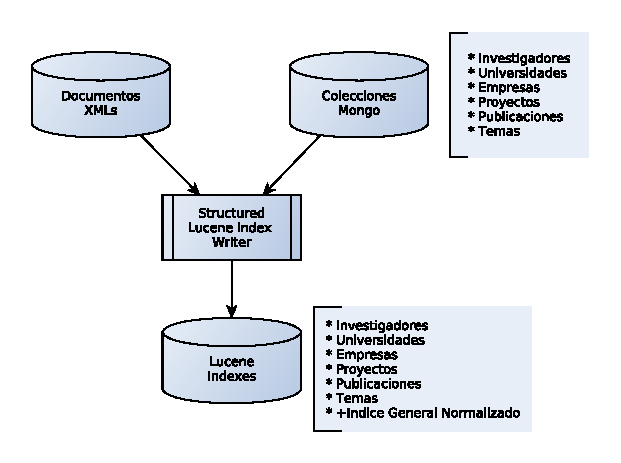
\includegraphics{graficos/LuceneIndexWriterEstructurado}
   \caption{Lucene Index Writer para datos del proyecto Mitic}
   \label{fig:LuceneIndexWriterEstructurado}
 \end{figure}

\begin{center}
\begin{table}
\centering
\begin{tabular}{|  l | l |}
\hline
\multicolumn{2}{|c|}{Totales} \\ \hline
Colección & Total \\ \hline
Universidades & 63 \\ \hline 
Empresas & 1561\\ \hline 
Investigadores & 1233\\ \hline 
Proyectos & 1247\\ \hline 
Publicaciones & 11821\\ \hline
Temas & 2267\\ \hline  
\end{tabular}
\caption{Totales por colección}
\label{table:temas}
\end{table}
\end{center}

En el Apéndice \allref{chap:db} describimos y ejemplificamos con valores el tipo de datos de los atributos de las seis colecciones, y comentamos los atributos que eliminamos por ser meta-datos o estar vacíos. El modelo de datos final es como sigue: \newline

\textit{Universidades(Id, Canónico, Nombre, Dirección, Página)} \newline

\textit{Investigadores(Id, Nombre y Apellido, Fecha Nacimiento, E-mail,   Teléfono,   Titulo,  Centro, Lugares Trabajo, Tema ,  Url Personal)} \newline

\textit{Empresas(Id, Nombre, Año Fundación, Cantidad Empleados, Domicilio, Ciudad, Provincia, ID LinkedIn, Teléfono, Website url, Descripción, Especialidades)} \newline

\textit{Proyectos(Id, Titulo, Keywords, Director, Investigadores Nombre, Entidad Benefactora, Instrumento, Descripción, Año, Año Hasta)} \newline

\textit{Temas(Id, Nombre)} \newline

\textit{Publicaciones(Id, Titulo, Keywords, Investigadores Nombre, Journal, Resumen, Url Doc)}


Siguiendo a \cite{QADB1} utilizamos $D$ para referir a la base de datos. El conjunto de colecciones $c$, de seis elementos, es \{universidades, investigadores, empresas, publicaciones, proyectos y temática\}, el conjunto de atributos $a$ es \{Canónico, Nombre, Dirección, Página, Nombre y Apellido, Fecha Nacimiento, email, Teléfono, Título, Centro, Lugares Trabajo, Tema , Url Personal, Año Fundación, Cantidad Empleados, Domicilio, Ciudad, Provincia, ID LinkedIn, Teléfono, Website url, Descripción, Especialidades, Keywords, Director, Investigadores Nombre, Entidad Benefactora, Instrumento, Año, Año Hasta, Journal, Resumen, Url Doc\}, de cardinalidad 33 y el conjunto de valores $v$ contiene cada dato de información independiente de la base de datos. La suma de estos tres conjuntos determinan el espacio de elementos $E$ que es el material básico para el modelo teórico. En nuestro modelo utilizaremos, constantemente, la noción de \textit{entidad}. Una entidad es el equivalente a una \textit{fila} en una base de datos relacional. El investigador Jorge Pérez, la Universidad de Mar de Ajó y el tema Inteligencia Artificial son ejemplos de entidades. Llamaremos $e$ al conjunto de entidades.

En lo que resta de esta sección (\ref{subsec:modelos-db}) discutiremos la implementación de distintas funciones del modelo teórico sobre este modelo de datos.

% \begin{figure}[H]
%   \centering
%     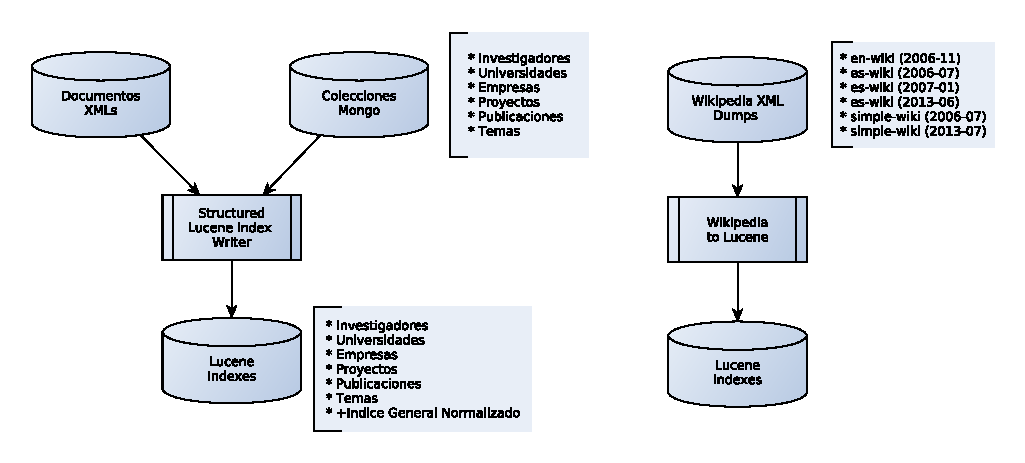
\includegraphics[scale=0.86]{graficos/LuceneWritersJuntos}
%   \caption{Creación de Indices}
%   \label{fig:LuceneIndexWriterBoth}
% \end{figure}



%Es importante notar que en la base de datos no hay relaciones de muchos a muchos: todas son de uno a muchos o de uno a uno. Estas relaciones, en un nivel técnico, se implementan como un atributo en una entidad refiriendo a la otra. Por ejemplo, para la relación \dq{Investigador}, la columna \dq{Universidad ID} refiere a una universidad en la relación \dq{Universidades}. A fin de acotar la implementación y de adecuar la base de datos al modelo simple expuesto en \ref{sec:closed-domain}, decidimos considerar, para estas relaciones, solamente un grado de indirección. Por ejemplo, consideramos la pregunta \dq{¿En qué universidad trabaja Juan Perez?}, pero no \dq{¿En qué ciudad está la universidad en la que trabaja Juan Perez?}). De esta manera, la algoritmia necesaria para tratar una relación es análoga a la de tratar un atributo.




\subsection{Interfaz de servicios}
\label{subsec:modelos-db}

Para la implementación del módulo de acceso a la información reutilizamos el modelo de datos escrito en Java del grafo de entidades que obtuvimos de los investigadores del proyecto Mitic. A estos modelos les agregamos soporte para su representación como documento dentro de los índices. Por ejemplo, el modelo para la entidad \dq{Universidad de Buenos Aires}, además de persistirse en la colección de universidades de la base de datos de MongoDB, también dispone de una representación como documento en su índice lucene particular (el índice de universidades) y otra en el índice general. A nivel colecciones, cada entidad dispone de un representante que maneja el acceso su información. A partir de estos manejadores de colecciones creamos la interfaz \emph{KnowlegdeBase}, que toma responsabilidades genéricas sobre su colección.

Los atributos relacionales son: {\color{red}ESTOS}. %terminar esto o sacar.

Por otro lado, las adyacencias del grafo pueden relacionar, en principio, a cualquier entidad con cualquier otra entidad y sin ninguna especificación de la naturaleza de la relación. Las adyacencias representan la relación general \dq{se relaciona con} sin especificar un modo puntual como sería \dq{trabaja en} o \dq{estudió con}, etc. 

Las $KnowledgeBase$ de las seis entidad y el índice general están, a su vez, controlados un $KnowlegdeManager$, que es la interfaz del módulo que maneja la base de conocimiento. 

El $KnowledgeManager$ ofrece diferentes servicios de verificación de entidades. Para un conjunto de tokens {\color{red}anotados} cualquiera, este módulo puede decidir, con un cierto grado de confianza, los siguientes problemas:

\begin{itemize}
  \item Si el conjunto de tokens se traduce a una colección del modelo de datos, es decir, si se están nombrando \dblquote{Investigadores} o \dblquote{Universidades} como clase de entidades.
  \item Si el conjunto de tokens se traduce como un atributo o una relación válida para una colección de entidades.
  \item Si el conjunto de tokens se traduce como una entidad dentro del modelo de datos: una universidad, una empresa, un investigador, un proyecto, una publicación o una temática
  \item Si el conjunto de tokens se traduce como un valor de alguna entidad del modelo
\end{itemize}

Estos servicios % te referís a lo que mencionás como problemas? no lo cambies porque no se entiene la correferencia.
 cubren lo que en \ref{subsec:closed-domain} definimos como función de traducción, \tradqd. Para la implementación de estos servicios, en todos los casos, reificamos la noción de comparación (Ver Apéndice \allref{sec:comparadores}), asignando distintos comparadores a los elementos. 

Para resolver los primeros dos items definimos, para cada colección $c_i \in c$ un diccionario de sinónimos a mano ($syn(c_i)$) y también para cada atributo $a_j \in a$ definimos diccionarios de sinónimos $syn(a_j)$. Estos diccionarios podrían ampliarse, en un futuro, incorporando un tesauro como Wordnet, o diferentes recursos automáticos de sinonimias. Por otro lado, definimos diccionarios solo para el español y sería interesante incorporar un proceso de traducción -o diccionarios diferentes- para cada idioma que el sistema busque soportar- lo cual es una tarea costosa. Con respecto a las relaciones entre entidades, para los atributos relacionales normales utilizamos la misma técnica de verificación por lookup en un diccionario, mientras que para las adyacencias consideramos diferentes casos en función de la entidad nombrada.

Para abordar la detección de entidades, marcamos diferentes atributos como identificadores. \textit{Universidades(Canónico, Nombre)}, \textit{Investigadores(Nombre y Apellido,E-mail)}, \textit{Empresas(Nombre)}, \textit{Proyectos(Titulo)}, \textit{Temas(Nombre)}, \textit{Publicaciones(Titulo)}. Consideramos que un conjunto de tokens se traduce como una entidad si se traduce como el valor de un atributo marcado como identificatorio. 

Finalmente, para la comparación de conjunto de tokens con valores, introdujimos diferentes comparadores, más o menos complejos, para los distintos atributos. 

El funcionamiento del $KnowlegdeManager$ será ilustrado en lo que resta del capitulo ya que resultará más claro introducir la motivación de ciertas definiciones en el contexto de su uso concreto. En la proxima sección (\ref{sec:qp-mitic}) veremos como se etiqueta la pregunta haciendo uso de herramientas de procesamiento de lenguaje y de algunos de los servicios recién enumerados y en la sección subsiguiente (\ref{sec:ar-mitic}) veremos nuevamente a este módulo como proveedor de servicios del proceso que decide la tratabilidad de la pregunta y, si es el caso, genera y presenta la respuesta final.

\begin{figure}[H]
  \centering
    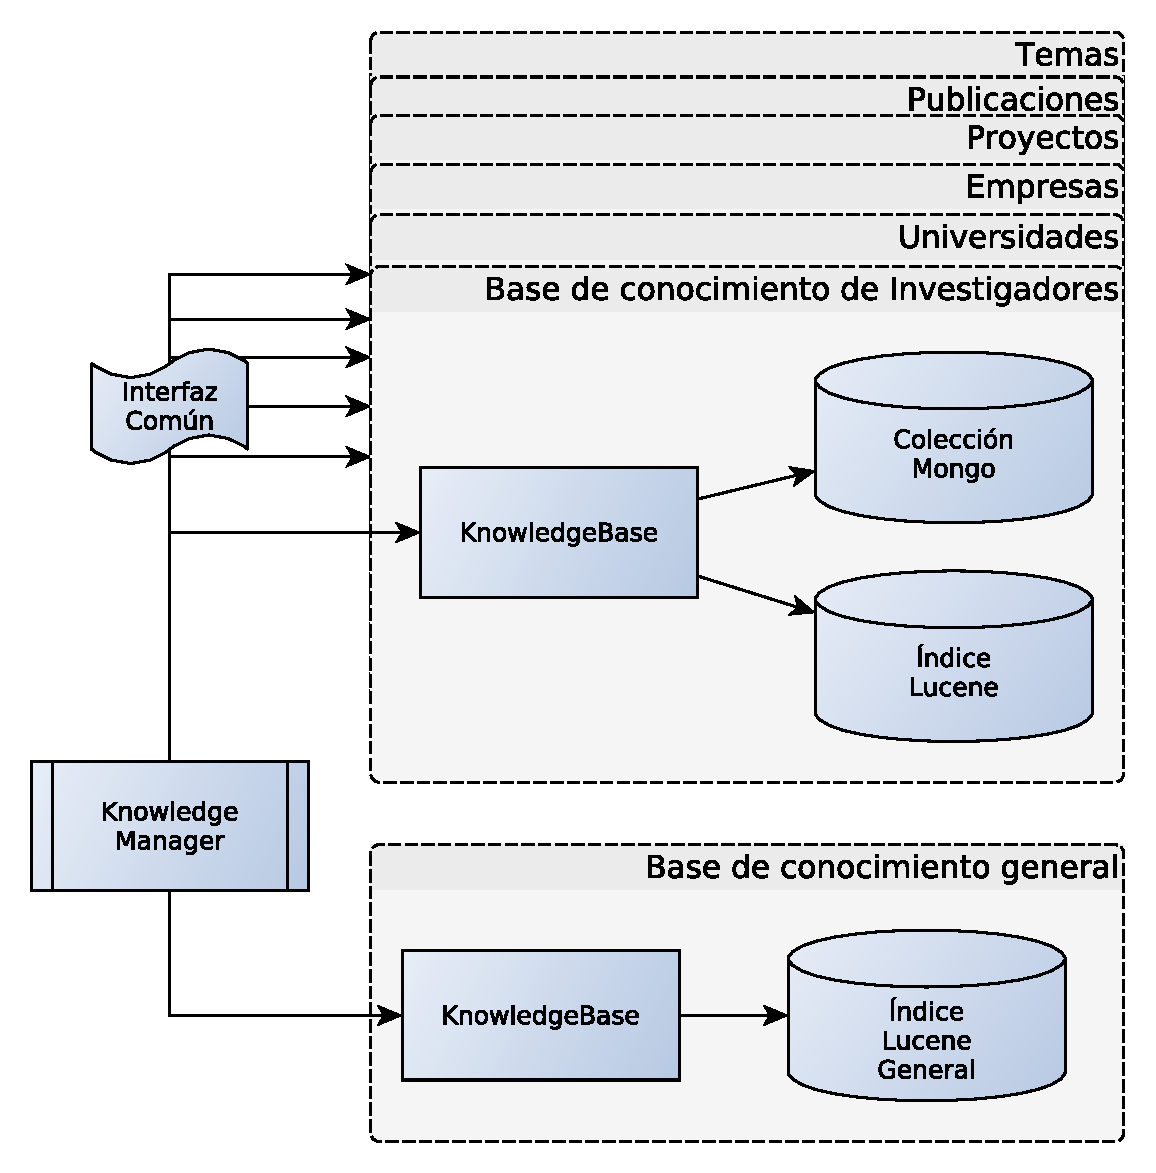
\includegraphics[scale=0.5]{graficos/KnowledgeManager}
  \caption{Base de Conocimiento de grafo de TICs}
  \label{fig:KnowledgeManager}
\end{figure}

\section{Anotado de la pregunta}
\label{sec:qp-mitic}

%% Debería haber algún ejemplo acá del resultado.

En este paso se realizan diferentes análisis lingüísticos de la pregunta. El resultado son distintas características asociadas a la pregunta (anotaciones) y distintas entidades semánticas reconocidas útiles para el proceso de generación de respuestas. 
Las herramientas de procesamiento de lenguaje natural que utilizamos en nuestra implementación incluyen: detección de lenguaje, extracción y verificación de entidades nombradas (NER), de verbos, sustantivos, qwords (qué, quién, cómo) (POS), análisis de n-gramas y categorización por tipo de pregunta (QC).
Con ellas implementamos diferentes módulos que anotan los tokens y la pregunta original y la dejan preparada para ser consumida por el módulo de generación de respuestas. En lo que sigue de esta sección, veremos los siguientes módulos:

\begin{itemize}
\item Detección de idioma 
\item Detección y verificación de entidades nombradas
\item Análisis gramatical
\item Clasificación del tipo de pregunta
\end{itemize}

Si bien es cierto que el segundo ítem está basado principalmente en NER-tagging, el tercero en POS-tagging y el cuarto en Question Classification, 
cada uno de estos pasos utiliza estas herramientas de diferentes maneras. Por ejemplo, para la detección y verificación de entidades, además del NER-tagger también utilizamos la base de conocimiento y el análisis gramatical y, para el español, la clasificación del tipo de pregunta se hace apoyándose en las qwords identificadas por el POS-tagger.

\subsection{Detección de idioma}

Uno de los objetivos iniciales del sistema es que sea capaz de responder preguntas en inglés y en español. En el modelo que describiremos en el próximo capítulo, el módulo de detección de idiomas no es utilizado porque en los problemas no se evalúa esta detección de idiomas. Los archivos de preguntas están separadas por idioma y no se espera que el idioma se infiera a partir de los textos de las preguntas, sino que es un dato dado al sistema participante. En este modelo, en cambio, no está disponible ninguna información sobre el idioma de la pregunta, por lo que es necesario detectarlo. El módulo de detección de idiomas de este sistema utiliza dos librerías distintas: el módulo de detección de idiomas de Freeling y una librería especializada de Cybozu Labs. (Ver apéndices \allref{sec:freeling} y \allref{sec:cybozu} para más información).

Ambos permiten priorizar la detección de ciertos idiomas sobre otros desde su configuración.
De esta manera podemos forzarlos a identificar sólo los idiomas esperados en nuestro dominio. 
Ambos fueron configurados para detectar inglés y español para mejorar la confiabilidad,
pero pueden habilitarse más idiomas de ser necesario y funcionan correctamente. 

\begin{figure}
  \centering
    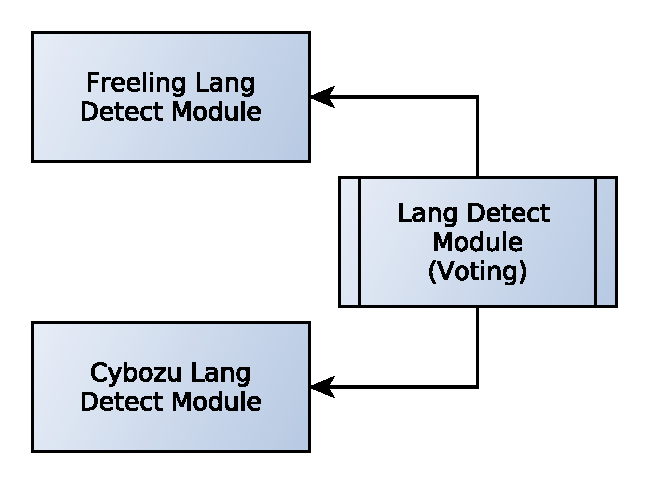
\includegraphics[scale=0.5]{graficos/LangDetect}
  \caption{Módulo de Detección de Idiomas}
  \label{fig:LangDetect}
\end{figure}


El módulo de detección simplemente evalúa ambos algoritmos y 
decide el resultado con un cierto grado de confianza. En caso de existir un empate, se 
prioriza la opción de Cybozu labs que en la práctica dio resultados más exactos.

De todos modos, el problema ``detección de idioma" no introduce mayores complicaciones y parece un problema bien resulto.
Es decir, la mayoría de las veces ambos módulos responden lo mismo y de modo correcto.
Sin embargo, para ciertos casos bordes molestos (pero lamentablemente frecuentes)
el detector de Cybozu resultó funcionar mejor. Por ejemplo, está el caso de la pregunta formulada en inglés pero acerca de una entidad nombrada en español: 
``Where is located the Universidad de Buenos Aires?". Este problema está particularmente presente en el procesamiento de preguntas, dado que son textos cortos en los que una construcción sustantivada en otro idioma puede desequilibrar erróneamente la balanza. 

A continuación presentamos algunos ejemplos que ilustran el funcionamiento de ambas librerías y el resultado final de nuestro módulo en estos casos:

\begin{center}
\begin{tabular}{| p {8cm} | l | l | l |}
\hline
Texto & Freeling & Cybozu & Resultado \\ \hline
¿Dónde queda la Universidad de Buenos Aires? & es & es & es \\ \hline
Where is located the University of Buenos Aires? & en & en & en \\ \hline
Where is located the Universidad de Buenos Aires? & en & en & en \\ \hline
Where is located Universidad de Buenos Aires? &  {\color{red}es} & en & en \\ \hline
Quién es Carolina Fernandez? & es & es & es \\ \hline
Who is Carolina Fernandez? &  {\color{red}none} & en & en \\ \hline
Quién es John McCain? & {\color{red}none} & es & es \\ \hline
Who is John McCain? & en & en & en \\ \hline
Dónde vive John McCain y por qué vive allí? & es & es & es \\ \hline
Where does Carolina Fernandez live and why does she lives there? & en & en & en \\ \hline
\end{tabular}
\end{center}

\subsection{Entidades nombradas}
\label{subsec:impl-ner}

Para la detección de entidades utilizamos la clase simple de detección (NER) y clasificación (NEC) de entidades de Freeling y el NERC de Stanford (ver \allref{sec:freeling} y \allref{sec:stanford-both}). Las herramientas de Stanford en general superan a las de Freeling -al igual que el detector de idiomas de Cybozu-, pero sólo sirven para inglés. La clasificación utilizada por ambos es la más general de las comentadas en \allref{subsec:nerc}: persona, lugar, organización y otros. 

Veamos algunos ejemplos de funcionamiento de los módulos de detección de entidades. 
%% Esta tabla no parece tener sentido acá sacarla o poner lo que corresponda.

\begin{center}
\begin{tabular}{| p {8cm} | l | l | l |}
\hline
Texto & Freeling & Stanford & Resultado \\ \hline
¿Dónde queda la Universidad de Buenos Aires? & es & es & es \\ \hline
Where is located the University of Buenos Aires? & en & en & en \\ \hline
Where is located the Universidad de Buenos Aires? & en & en & en \\ \hline
Where is located Universidad de Buenos Aires? &  {\color{red}es} & en & en \\ \hline
Quién es Carolina Fernandez? & es & es & es \\ \hline
Who is Carolina Fernandez? &  {\color{red}none} & en & en \\ \hline
Quién es John McCain? & {\color{red}none} & es & es \\ \hline
Who is John McCain? & en & en & en \\ \hline
Dónde vive John McCain y por qué vive allí? & es & es & es \\ \hline
Where does Carolina Fernandez live and why does she lives there? & en & en & en \\ \hline
\end{tabular}
\end{center}

\medskip

Mientras la detección de entidades para el modelo que veremos en el capitulo siguiente se detiene en el reconocimiento de entidades nombradas a nivel lingüístico, para el sistema estructurado el proceso es un poco más complejo. Esto se debe a que en este caso la detección de entidades es esencial. Si en el proceso de anotado de la pregunta no se logra identificar alguna entidad reconocida por el modelo de datos, entonces se está muy lejos de encontrar una respuesta. Por eso, además de utilizar los módulos NER recién mencionado, agregamos otros algoritmos de detección y, también, verificación de entidades. 

En principio, verificamos la o las entidades nombradas reconocidas contra la base de conocimiento. El $KnowledgeManager$ ofrece diferentes servicios de verificación de entidades. Para una cadena de tokens cualquiera, este módulo puede decidir, con un cierto grado de confianza, si:

\begin{itemize}
  \item La cadena de tokens es una entidad dentro del modelo de datos. Esto incluye:
    \begin{itemize}
      \item Es una entidad del modelo de datos: una universidad, una empresa, un investigador, un proyecto, una publicación o una temática
      \item Es una entidad inferida: una ciudad, una provincia, un centro de investigación, un lugar de trabajo
    \end{itemize}
  \item La cadena es una colección del modelo de datos, es decir, si se están nombrando \dblquote{Investigadores} o \dblquote{Universidades} como clase de entidades.
  \item La cadena es un atributo o una relación de una clase. (nombre de investigador)
\end{itemize}

Parte importante del trabajo para este esquema es lograr identificar este tipo de entidades lingüísticas, por lo que además de verificar los resultados del proceso de NER-tagging, también generamos otras cadenas de input. Notar además que los nombres de clase y de atributos de clase no tendrían por que ser reconocidas por el NER-tagger. Por ejemplo, para ``¿Qué investigadores trabajan en Córdoba?", \dblquote{investigadores} está haciendo referencia al nombre de una clase pero no es el tipo de entidades lingüísticas que detecta un NER-tagger. 

Por estas razones, generamos más entidades lingüísticas posibles además de las entidades detectadas por los NER-taggers. Una vez que todas las entidades nombradas fueron verificadas, generamos n-gramas sobre el resto de la pregunta para chequear por más tokens reconocibles. Configuramos la generación de n-gramas de 1 a 3, con ciertos filtros para no verificar construcciones que no representan entidades de manera trivial. Por ejemplo: dejamos sólo los unigramas que cumplan el rol de sustantivos, eliminamos bigramas que sean un sustantivo y una acción, salteamos NERs ya reconocidas, entre otros.


\subsection{Análisis gramatical}
\label{subsec:impl-pos}
De las diferentes etiquetas que generan los POS-taggers, en este modelo distinguimos los verbos, los sustantivos, las qwords y las palabras triviales. 
Las palabras etiquetadas cumplen distintos roles a lo largo del proceso de generación de respuestas. Como señalamos recién, los n-gramas que se verifican contra la base de datos están filtrados por los roles gramaticales de sus tokens. Por otro lado, a la hora de generar el tipo de pregunta para una pregunta en español, utilizamos, como mecanismo ad-hoc, las qwords. 

\begin{center}
\begin{tabular}{| l | l |}
\hline
Clase & Ejemplos\\ \hline
qword  & qué, quién, cómo, dónde, cuándo\\ \hline
verbo & trabaja, trabajar, trabajando \\ \hline
trivial  & lo, a, de, y \\ \hline
sustantivos  & universidad, impresora, álgebra \\ \hline
\end{tabular}
\end{center}

Los usos más intensivos de estas etiquetas son el filtrado de n-gramas que mencionamos recién (\allref{subsec:impl-ner}), y un algoritmo ad-hoc de etiquetado de Q-Type para el caso español (es el próximo tema a discutir en \allref{subsec:qtype}) y, finalmente, son utilizados en la generación de respuestas, para jerarquizar  tokens de la pregunta al vincularlos con elementos de la base de datos.

\subsection{Clasificación}
\label{subsec:qtype}
Para clasificar la pregunta según su tipo de respuesta esperada utilizamos el Question Classifier de Stanford, tomando la configuración de Qanus. Este clasificador arroja una clase y una subclase (ver \allref{sec:stanford-qc} para una lista detallada de las posibles clases) y un grado de confianza para esta asignación. A continuación presentamos algunos ejemplos que ilustran estos resultados.

\begin{center}
\begin{tabular}{| l | l | l |}
\hline
Pregunta & Clase y Subclase & Confianza\\ \hline 
What's his name? & HUM:ind & 0.74 \\ \hline 
Where do you come from? & DESC:desc & 0.62 \\ \hline 
What's your phone number? & NUM:code & 0.63 \\ \hline 
How old are you? & NUM:period & 0.78 \\ \hline 
When were you born? & NUM:date & 0.99 \\ \hline 
What does he look like? & DESC:desc & 0.82 \\ \hline 
\end{tabular}
\end{center}

Sin embargo, como ya señalamos oportunamente (ver \allref{subsec:qc}), no existen herramientas de clasificación de preguntas para el idioma español. Por esta razón, escribimos un clasificador básico basado en reglas escritas a mano sobre qwords. Las qwords, como vimos, son palabras clave de las preguntas que señalan el tipo de respuesta. Por ejemplo: una pregunta que comienza con `Cuándo' tendrá como tipo de respuesta una fecha, un tiempo, etc. Para este modelo, definimos una serie acotada de categorías de tipo de respuesta esperadas y unificamos los resultados del clasificador de Stanford y nuestras reglas sobre qwords para español para unificar el código. Estas categorías son:  Who, Whom, Where, Which,  When,  What y Other. Es decir: Quién, Quiénes, Dónde, Cuál, Cuándo, Qué y otros. Las clases y subclases del clasificador de Stanford se mapearon a estas categorías que coinciden con los resultados de las reglas escritas a mano para el español. 


\section{Generación de Respuestas}
\label{sec:ar-mitic}
\horrible
%% Esta parte hay que mejorarla y poner algún ejemplo, no está ``horrible''

Una vez etiquetados todos los tokens de la pregunta, se procede a marcar como procesadas las ``marcadores sintácticos", mediante un filtro que incorpora stopwords por idioma y algunas clases de pos-tags (como proposiciones, pronombres y algunos conectores). Si al etiquetar la pregunta no se logró identificar ninguna entidad del modelo, entonces será difícil avanzar. Como vimos recién, la fase de procesamiento de la pregunta para el caso estructurado excede por mucho la mera anotación lingüística: al finalizar el etiquetado deberíamos disponer de al menos una entidad reconocida por el modelo. Por otro lado, durante la fase de etiquetado cada palabra se marca como procesada. Como acabamos de señalar, al finalizar este proceso se marcan también como procesados ciertos tokens triviales. En lugar de exigir una traducción completa de la pregunta, aplicamos la siguiente regla: si no ha logrado etiquetar una cierta cantidad de tokens (más del 80\%), entonces se considera que no tiene sentido dar por ``comprendida" la pregunta y se procede a un segundo análisis, computacionalmente más costoso y además más inexacto, en el que se intenta encontrar alguna entidad con otros métodos que enunciaremos en breve. En caso de encontrarse una entidad, entonces el flujo del programa retorna al curso de análisis estructurado. Si esto no ocurre, se devuelve la lista de entidades (documentos) que el índice lucene general devuelve para la pregunta original interpretada como una query normal de information retrieval. Este caso, si bien retorna información, es un caso de falla de procesamiento. Esta lista de documentos viene acompañada de un mensaje del tipo: \dblquote{No se logró interpretar su pregunta} y, en un trabajo futuro, podría incorporar un sistema de recomendaciones e idas y vueltas con el usuario (¿Quiso decir...?).

Si, en cambio, el threshold de tokens es alcanzado, entonces se avanza al siguiente paso, en el que se distingue según la cantidad de entidades del modelo reconocidas. Por entidades del modelo entenderemos, aquí, entidades internas, objetos, no nombres de clase o de atributos ni valores. Distinguimos estos tres casos: `ninguna entidad reconocida', `una entidad reconocida', `más de una entidad reconocida'.



\begin{figure}[H]
  \centering
    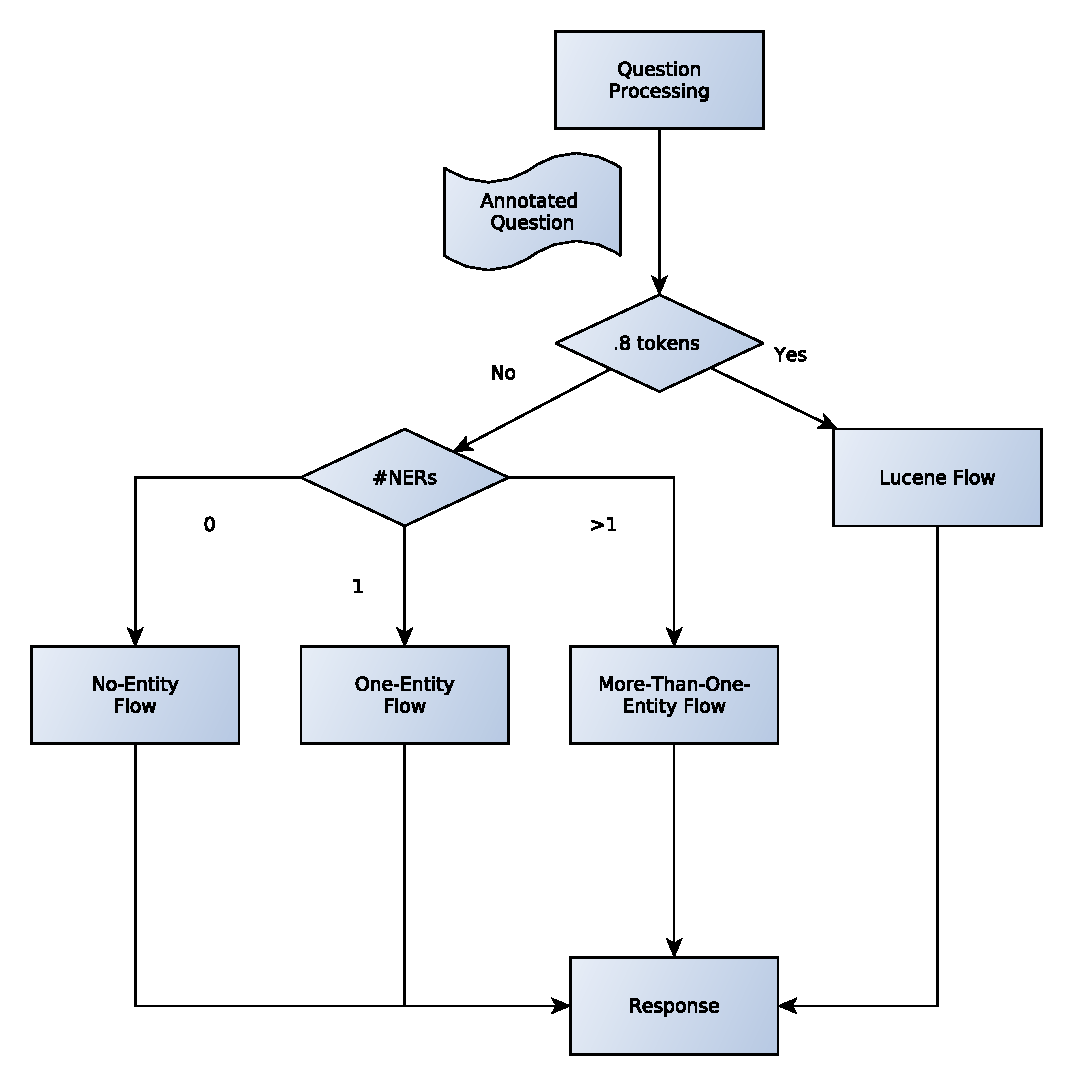
\includegraphics[scale=0.5]{graficos/AnswerRetrievalFlowEstructurado}
  \caption{Flow para la Generación de Respuestas - Estructurado}
  \label{fig:AnswerRetrievalFlowEstructurado}
\end{figure}

\subsubsection*{Ninguna o más de una entidad}
En el caso en el que no se haya identificado ninguna entidad del modelo quedan diferentes posibilidades, que se verifican en orden secuencial en base a nombres de colección, nombres de atributos, tipo de respuesta esperada y verbos. Los casos contemplados son: la pregunta por un campo de una colección (por ejemplo: direcciones de empresas en buenos aires) o por listas de entidades de una colección (investigadores de capital federal). Los diferentes casos son reglas de código escritas a mano. En todos los casos, si no se dan las condiciones para seguir especificando la dirección de la respuesta, se genera un respuesta ad-hoc con datos rankeados según el índice invertido, especificando de modo estructurado el camino recorrido hasta el momento. Por ejemplo, si se identifica que se pregunta por `investigadores' pero no es posible decidir ninguna especificación más (de capital federal, que hayan publicado en 2008, etc) entonces se retorna una lista de investigadores rankeada según el índice invertido `investigadores' con el resto de los datos de la pregunta. 

Por otro lado, si hay más de una entidad reconocida entonces hay sólo algunos casos posibles de relaciones entre ellas que pueden ser respuestas, que también se reflejan como caso de código. Finalmente, si no es posible identificar ninguno de estos caso, se toma un camino similar al mecanismo ad-hoc basado en information retrieval.


\subsubsection*{Una entidad}
El mejor caso es aquél en el que se reconoció una entidad y otros datos lingüísticos que permitan especificar qué se está preguntando. Al especificar acerca de qué/quién resulta mucho más sencillo canalizar qué se está preguntando. Los modelos que representan objetos (ver \allref{subsec:modelos-db}) son subclases de $NodoBase$, el cual representa una entidad en abstracto. Una entidad sabe responder preguntas acerca de ella. Para esto, utiliza las anotaciones de verbos, atributos nombrados y qwords para identificar qué se está preguntando. La pregunta puede responderse con un atributo o con una relación. Los distintos atributos de las distintas entidades se corresponden con verbos y con tipos de respuesta esperada. 

[[Detalle de casos y combinaciones de verbos + tipo de respuesta esperada + atributo]]
[[Ejemplos]]

%No se entiende esto último. Toda esta sección hay que mejorarla con ejemplos en lo posible.